\documentclass[12pt]{article}
\usepackage{natbib}
\usepackage{url}
\usepackage{amsmath}
\usepackage{graphicx}
\graphicspath{{fig/}}
\usepackage{parskip}
\usepackage{adjustbox}
\usepackage{fancyhdr}
\usepackage{commath}%定义d
\usepackage[UTF8,heading=true]{ctex}
\usepackage{bm}
\usepackage{titlesec}
\usepackage{caption}
\usepackage{paralist}
\usepackage{multirow}
\usepackage{booktabs} % To thicken table lines
\usepackage{titletoc}
\usepackage{diagbox}
\usepackage{bm}
\usepackage{autobreak}
\usepackage{authblk}
\usepackage{indentfirst}
\usepackage{float}
\usepackage{amsthm}
\usepackage{fontspec}
\usepackage{color}
%\usepackage{txfonts} %设置字体为times new roman
\usepackage{lettrine}
\usepackage{nameref}
%\usepackage[nottoc]{tocbibind}
\usepackage{amssymb}%font
\usepackage{lipsum}%make test words
\usepackage{picinpar}%words around the picture
\usepackage[all]{xy}%draw arrow
\usepackage{asymptote}%draw picture
\usepackage[perpage]{footmisc}%脚注每页清零
\usepackage[cmyk]{xcolor}

% \geometry{bottom=2.5cm,left=2cm,right=2cm,top=2.5cm}
\newcommand{\crefrangeconjunction}{ - }
\setlength{\parindent}{2em}

\ctexset{today=big}%日期类型设置


% ======================================
% = Color de la Universidad de Sevilla =
% ======================================
\usepackage{tikz}
\definecolor{PKUred}{cmyk}{0,1,1,0.45}
%超链接设置
\usepackage[breaklinks,colorlinks,linkcolor=PKUred,citecolor=PKUred,pagebackref,urlcolor=black]{hyperref}
\usepackage{cleveref}


\renewcommand*\footnoterule{%
    \vspace*{-3pt}%
    {\color{PKUred}\hrule width 2in height 0.4pt}%
    \vspace*{2.6pt}%
}





% %%% Equation and float numbering
% \numberwithin{equation}{section}		% Equationnumbering: section.eq#
% \numberwithin{figure}{section}			% Figurenumbering: section.fig#
% \numberwithin{table}{section}				% Tablenumbering: section.tab#


%代码设置
\usepackage{listings}
\usepackage{fontspec} % 定制字体
\newfontfamily\menlo{Menlo}
\usepackage{xcolor} % 定制颜色
\definecolor{mygreen}{rgb}{0,0.6,0}
\definecolor{mygray}{rgb}{0.5,0.5,0.5}
\definecolor{mymauve}{rgb}{0.58,0,0.82}
\lstset{ %
backgroundcolor=\color{white},      % choose the background color
basicstyle=\footnotesize\ttfamily,  % size of fonts used for the code
columns=fullflexible,
tabsize=4,
breaklines=true,               % automatic line breaking only at whitespace
captionpos=b,                  % sets the caption-position to bottom
commentstyle=\color{mygreen},  % comment style
escapeinside={\%*}{*)},        % if you want to add LaTeX within your code
keywordstyle=\color{blue},     % keyword style
stringstyle=\color{mymauve}\ttfamily,  % string literal style
frame=single,
rulesepcolor=\color{red!20!green!20!blue!20},
% identifierstyle=\color{red},
language=c++,
xleftmargin=4em,xrightmargin=2em, aboveskip=1em,
framexleftmargin=2em,
numbers=left
}

%脚注
\renewcommand\thefootnote{\fnsymbol{footnote}}

%定义常数i、e、积分符号d
\newcommand\mi{\mathrm{i}}
\newcommand\me{\mathrm{e}}

%%% Maketitle metadata
\newcommand{\horrule}[1]{\rule{\linewidth}{#1}} 	% Horizontal rule
\newcommand{\tabincell}[2]{\begin{tabular}{@{}#1@{}}#2\end{tabular}}

\newcommand{\chuhao}{\fontsize{42pt}{\baselineskip}\selectfont}
\newcommand{\xiaochuhao}{\fontsize{36pt}{\baselineskip}\selectfont}
\newcommand{\yihao}{\fontsize{28pt}{\baselineskip}\selectfont}
\newcommand{\erhao}{\fontsize{21pt}{\baselineskip}\selectfont}
\newcommand{\xiaoerhao}{\fontsize{18pt}{\baselineskip}\selectfont}
\newcommand{\sanhao}{\fontsize{15.75pt}{\baselineskip}\selectfont}
\newcommand{\sihao}{\fontsize{14pt}{\baselineskip}\selectfont}
\newcommand{\xiaosihao}{\fontsize{12pt}{\baselineskip}\selectfont}
\newcommand{\wuhao}{\fontsize{10.5pt}{\baselineskip}\selectfont}
\newcommand{\xiaowuhao}{\fontsize{9pt}{\baselineskip}\selectfont}
\newcommand{\liuhao}{\fontsize{7.875pt}{\baselineskip}\selectfont}
\newcommand{\qihao}{\fontsize{5.25pt}{\baselineskip}\selectfont}
\setcounter{secnumdepth}{2}
\usepackage{bm}
\usepackage{autobreak}
\usepackage{amsmath}
\setlength{\parindent}{2em}
\graphicspath{{fig/}}


%pdf文件设置
\hypersetup{
	pdfauthor={袁磊祺},
	pdftitle={高等应用数学作文}
}

\title{
		\vspace{-1in} 	
		\usefont{OT1}{bch}{b}{n}
		\normalfont \normalsize \textsc{\LARGE Peking University}\\[1cm] % Name of your university/college \\ [25pt]
		\horrule{0.5pt} \\[0.5cm]
		\huge \bfseries{从量子力学的发展来看应用数学} \\
		\horrule{2pt} \\[0.5cm]
}
\author{
		\normalfont 								\normalsize
		College of Engineering \quad 2001111690  \quad 袁磊祺\\	\normalsize
        \today
}
\date{}

\begin{document}

\input{setc.tex}

\maketitle

\section{经典理论受到挑战}

1900年4月27日,英国著名物理学家William Thomson(即开尔文男爵)在英国皇家学会发表了题为“在热和光动力理论上空的十九世纪的乌云”的演讲。他在回顾物理学所取得的伟大成就时说,物理大厦已经落成,现在,它的美丽而晴朗的天空却被两朵乌云笼罩了。”他所说的第二朵乌云,主要是指热学中的能量均分定则在气体比热以及热辐射能谱的理论解释中得出与实验不等的结果,其中尤以黑体辐射理论出现的“紫外灾难”最为突出。

维恩近似是用于描述热辐射光谱(通常称为黑体函数)的物理学定律。 该定律最早由威廉·维恩(Wilhelm Wien)于1896年推导。\cref{eq:1} 确实准确描述了物体的热辐射的短波长(高频)光谱,但未能准确拟合长波长(低频)辐射的实验数据。而Rayleigh-Jeans定律\cref{eq:3}在频率较大的地方增长到了负无穷。

\begin{equation}
	I(\lambda, T) = \frac{2 h c^2} {\lambda^5} e^{-\frac{hc}{\lambda kT}}
	\label{eq:1}
\end{equation}

\begin{equation}
	I(\lambda, T)= \frac{2 ckT}{\lambda^4}
	\label{eq:3}
\end{equation}

\begin{figure}[htp]
	\centering
	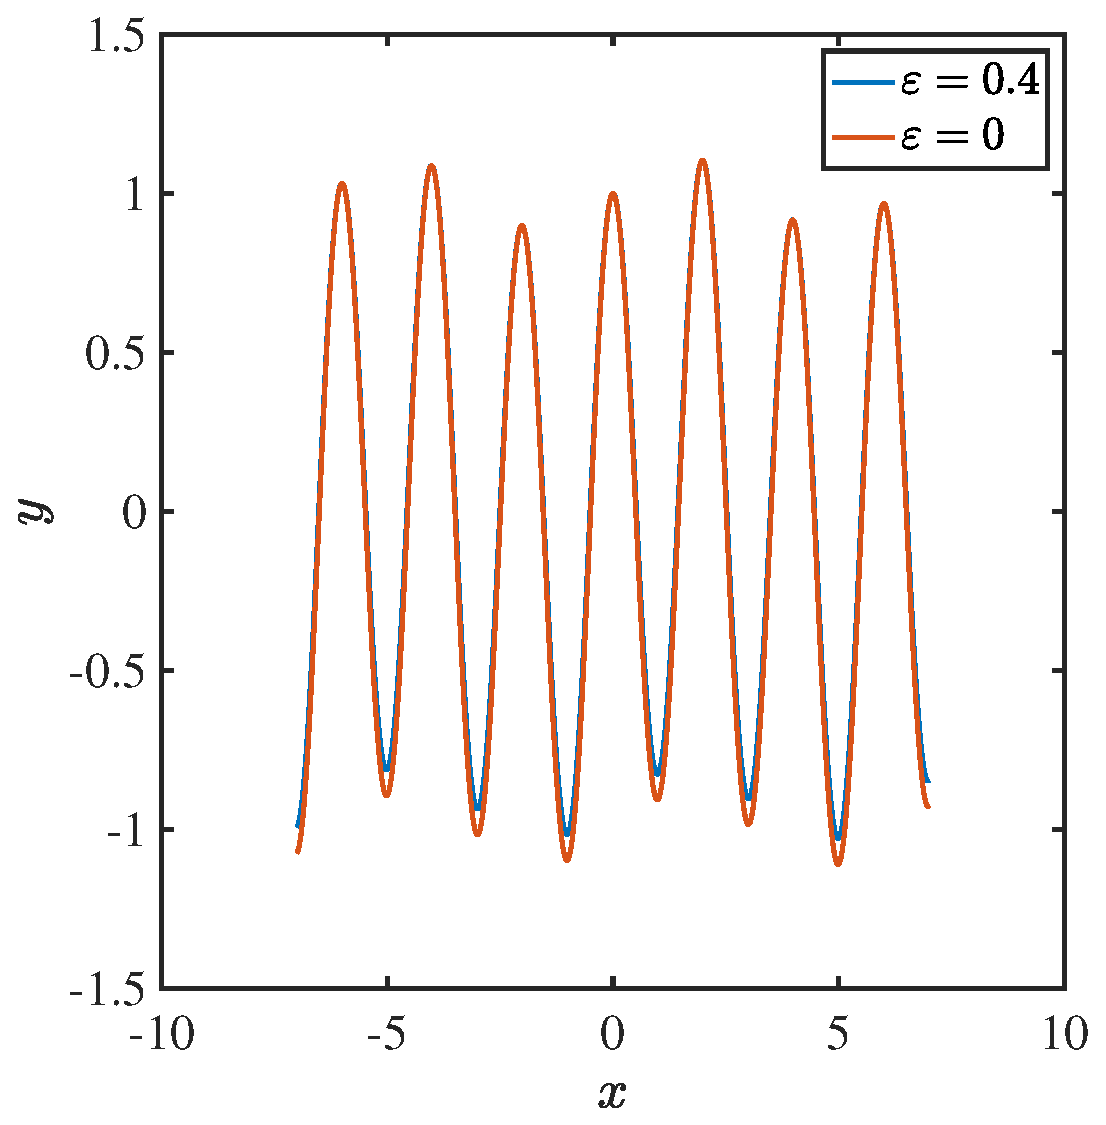
\includegraphics[width=9cm]{1}
	\caption{对于温度为5800 K的物体,将Wien分布定律与Rayleigh-Jeans定律和Planck定律进行比较。}
	\label{fig:1}
\end{figure}

\section{拟合与假设}

\subsection{黑体辐射}

传统公式的得来是有完整的理论体系作为支撑的,但是却与实际观测到的实验现象不符,这使得我们需要从原理上从新假设。普朗特的公式\cref{eq:2} 起初是半经验的,即利用内插法将适用于短波的维恩公式和适用于长波的瑞丽公式衔接起来。他目的就是拟合实验数据,这也就是第零步。

普朗特的公式和实验符合得很好。而为了从理论上论证它,普朗特提出了如下一个非同寻常的假设:谐振子能量的值只取某个基本单元的整数倍。当然这还没到建立方程的地步。

\begin{equation}
	I(\nu, T)=\frac{2 h \nu^3}{c^2} \frac{1}{e^{\frac{h \nu}{kT}}-1}
	\label{eq:2}
\end{equation}

\subsection{量子化}

19 世纪当化学家们在发现化学元素方面取得长足进展的同时,物理学 中光谱学的研究也硕果累累。物理学家们用光谱学方法帮助化学家发现多 种元素。这之所以可能 是因为原子气体的光谱是线状光谱,每种原子发射 或吸收特定波长(或者说频率)的谱线, 这些谱线成为辨认该种原子的“指纹”。

瑞士的一位中学教师巴尔末(J. J. Balmer)1884年发现巴尔末系的波长$\lambda$可纳入下列经验公式:
\begin{equation}
	\frac{1}{\lambda} = \widetilde{R}_H \left(\frac{1}{2^2}-\frac{1}{n^2}\right),
	\label{eq:20}
\end{equation}
其中$\widetilde{R}_H=109677.58$cm$^{_1}$, $n=3,4,5,\cdots$这个公式再经验不过了,但他非常好地总结了氢光谱的规律,但没有用到任何物理定理,没法说出前因后果。

之后玻尔提出了动量量子化的假设
\begin{equation}
	l_n=n\hbar,
	\label{eq:21}
\end{equation}
然后结合经典力学来描述电子的运动,得到原子的能量存在一系列定态
\begin{equation}
	E_n = - \frac{hc\widetilde{R}_H}{n^2}.
\end{equation}
\cref{eq:21} 可以较好地解释一些光谱,也结合了经典的理论,但是它没法预测别的情况,也没法解释量子力学遇到的其它问题。

这说明量子化背后还有更深刻的规律,有别的公式来推导出量子化条件。

\section{波函数和薛定谔方程}

为了描述微观世界,我们需要使用全新的思维方式、物理量和控制方程,而不再使用牛顿力学中的力、牛顿第二定理。在一些实验中,例如电子干涉、衍射实验,让一个一个的电子单独穿过双缝,最终却形成了干涉条纹,所以说电子并没有一个确定的轨迹,电子的运动遵循\textbf{不确定性原理},基于这个思想,产生了波函数,并找到了波函数满足的方程,薛定谔方程。从牛顿的确定性思维到量子力学的不确定性原理,正是机理上的转变,才跳出了电子有确定运动轨道的经典思路,并建模得到薛定谔方程。

我们用 $q$ 表示量子系统坐标的集合,用 $\mathrm{d} q$ 表示这组坐标的微分的乘积. $\mathrm{d} q$ 通常称为该系统位形空间中的一个体积元;对单粒子来讲, $\mathrm{d} q$ 等同于普通空间 中的一个体积元 $\mathrm{d} V .$
量子力学的数学表述基于这样的一个命题:在某一给定时刻。一个系统的状 态可以用一个确定的坐标函数 $\Psi(q)($ 通常为复函数 $)$ 来描述. 这个函数的模量 平方确定了坐标值的概率分布 : 对系统进行坐标测量时,测量所得诸值处于位形 空间的 $\mathrm{d} q$ 体积元内的概率等于 $|\Psi|^{2} \mathrm{~d} q . \Psi$ 函数称为该系统的波函数.

而波函数满足的方程就是薛定谔方程
\begin{equation}
	\mi \hbar \dot{\Psi} = \mathrm{\hat{H}}\Psi.
\end{equation}

\section{求解方程}

我们在使用近似方法时要注意
\begin{enumerate}
	\item 先要找到在某一区间内,方程占主导的几项.
	\item 舍去小量后要使得方程变简单.
	\item 求得的最终结果符合假设条件。
\end{enumerate}

对于氢原子,薛定谔方程可以化为
\begin{equation}
	\frac{\mathrm{d}^{2} R}{\mathrm{~d} r^{2}}+\frac{2}{r} \frac{\mathrm{d} R}{\mathrm{~d} r}-\frac{l(l+1)}{r^{2}} R+2\left(E+\frac{1}{r}\right) R=0,
\end{equation}
再求解可得
\begin{equation}
	E=-\frac{1}{2 n^{2}}, \quad n=1,2, \cdots.
\end{equation}

由此我们可以得到\cref{eq:20}其实就是电子的能级跃迁,同时,在求解过程中并没有用到角动量量子化的条件。建立方程,也就是应用数学的第一步。模型建立的原理有相似性、连续性、不变性原理,薛定谔方程一般来说并不是从更普适性的原理严格推导出来的,但可以从某些方面来解释,例如用描述波类似的方程来描述波函数,或者从变分原理(不变性)来推导出薛定谔方程。

薛定谔方程的精确解只有在少数简单情形下才能找到,对量子力学中的大 多数问题来讲,所得的方程过于复杂,很难精确解出.但是往往有这样的情形,在 所给问题的条件中,各量具有不同的数量级 ; 当我们把其中较小的量略去以后。 这个问题有可能变得十分简单,以致可以求出它的精确解.在这种情形下,求解 这个物理问题的第一步,是求出简化问题的精确解,第二步,是计算由于在简化 问题中略去了较小项而引起的误差. 计算这种误差的一般方法,称为微扰论.


我们假定某一给定物理系统的哈密顿量呈以下形式:
$$
\hat{H}=\hat{H}_{0}+\hat{V}
$$
式中的 $\hat{V}$ 是未受扰算符 $\hat{H}_{0}$ 的微小修正(或称微扰项).离散谱的微扰论问题,可按下列方式表述. 假定未受扰算符 $\hat{H}_{0}$ 的离散谱本 征值 $E_{n}^{(0)}$ 及其本征函数 $\psi^{(0)}$ 都是已知的, 即下列方程的精确解是已知的:
$$
\hat{H}_{0} \psi^{(0)}=E^{(0)} \psi^{(0)}
$$
现在欲求下列方程的近似解:
$$
\hat{H} \psi=\left(\hat{H}_{0}+\hat{V}\right) \psi=E \psi
$$
也就是求受扰算符 $\hat{H}$ 的本征值 $E_{n}$ 和本征函数 $\psi_{n}$ 所具有的近似表式.

\section{解释结果、现象}

波函数和薛定谔方程非常成功地解释了实验观测到的各种现象,例如之前提到的光谱,不光是氢原子,类氢离子,各种原子分子,电子云,杂化、能级分裂等等,同时,长度在取无限长的情况下,粒子的运动很自然地过度到了牛顿经典模型。一个好的模型,好的解释要有如下几个特征
\begin{enumerate}
	\item 能解释目前研究的某一个问题,例如氢原子光谱。
	\item 能预测别的情况,巴尔末经验公式和玻尔假设在遇到别的情况时就无法解释。
	\item 和已有理论能统一,牛顿力学在常规尺度上能很好地解释物体的运动,量子力学在考虑大尺度问题时能过度到牛顿力学。
	\item 一个好的理论应该基于更具有普适性、更高层的假设,例如这里的不确定性原理,跳出了传统思维框架,才取得了真正的成功。
\end{enumerate}

\section{总结}

通过这一学期的学习,我收获的不仅仅是知识,还有方法论,以及如何站在更高的角度看问题。物理世界有它内在的规律,这个规律可以用一句话,一个思想来说明,而描述它的最好的最好的方法就是应用数学,使用数学语言,从定性到定量,从观测到预测,通过数学的运算来更好地描述、预测事情,从而更深刻地理解物理世界。



\nocite{*}

\input{bib.tex}

\end{document}
